% SBG V8 -- IEEE Access manuscript, condensed working version (about 10 two-column pages).
% Built with tectonic (XeTeX) in a scratch copy; see BUILD_NOTE.txt. Source of truth: closeout/manuscript_final.
\documentclass{ieeeaccess}
\usepackage{cite}
\usepackage{amsmath,amssymb,amsfonts}
\usepackage{graphicx}
\usepackage{textcomp}
\usepackage{array}
\usepackage{multirow}
\usepackage{makecell}
\usepackage{xcolor}
\usepackage{url}
\usepackage{bm}
\usepackage{algorithm}
\usepackage[noend]{algpseudocode}
\usepackage{booktabs}
\makeatletter
\AtBeginDocument{\DeclareMathVersion{bold}
\SetSymbolFont{operators}{bold}{T1}{times}{b}{n}
\SetSymbolFont{NewLetters}{bold}{T1}{times}{b}{it}
\SetMathAlphabet{\mathrm}{bold}{T1}{times}{b}{n}
\SetMathAlphabet{\mathit}{bold}{T1}{times}{b}{it}
\SetMathAlphabet{\mathbf}{bold}{T1}{times}{b}{n}
\SetMathAlphabet{\mathtt}{bold}{OT1}{pcr}{b}{n}
\SetSymbolFont{symbols}{bold}{OMS}{cmsy}{b}{n}
\renewcommand\boldmath{\@nomath\boldmath\mathversion{bold}}}
\makeatother

% Shared notation. Verdict names follow the implementation (sbgv8/, sbgv7/).
\newcommand{\NDO}{NDO}
\newcommand{\DIV}{DIV}
\newcommand{\INS}{INS}
\newcommand{\NDOfull}{\texttt{NO\_DIVERGENCE\_OBSERVED}}
\newcommand{\DIVfull}{\texttt{DIVERGENT\_OBSERVABLE}}
\newcommand{\INSfull}{\texttt{INSUFFICIENT}}
\newcommand{\sbg}{SBG~V8}
\newcommand{\ers}{ERS}
\newcommand{\cec}{CEC}
\newcommand{\R}{\mathcal{R}}
\newcommand{\Rhat}{\widehat{\mathcal{R}}}
\newcommand{\obs}{\mathcal{O}}
\newcommand{\budget}{\mathcal{B}}
\newcommand{\Ev}{\mathcal{E}}
\newcommand{\prof}{\phi}
\newcommand{\cov}{\kappa}
\newcommand{\pp}{\,pp}
\newcommand{\code}[1]{\texttt{#1}}
% Breakable underscore and slash inside long code paths in tables.
\DeclareRobustCommand{\bus}{\textunderscore\allowbreak}
\newcommand{\bcode}[1]{{\def\_{\bus}\def\/{/\allowbreak}\texttt{#1}}}

\newcolumntype{L}[1]{>{\raggedright\arraybackslash}p{#1}}

% Theorem-like environments (plain LaTeX; the ieeeaccess class does not load amsthm).
\newtheorem{definition}{Definition}
\newtheorem{proposition}{Proposition}
\newtheorem{remark}{Remark}

% Ragged-right algorithm bodies (narrow IEEE column).
\usepackage{etoolbox}
\AtBeginEnvironment{algorithmic}{\raggedright}



\begin{document}
\history{}
\doi{}

\title{How Far Can a No-Divergence Verdict Be Trusted? False-Assurance Risk, Evidence Response Signatures, and a Pilot Study in Differential Regression Testing}

\author{\uppercase{Manas Sakthivel}}

\tfootnote{This work received no specific external funding.}

\markboth
{Sakthivel: How Far Can a No-Divergence Verdict Be Trusted?}
{Sakthivel: How Far Can a No-Divergence Verdict Be Trusted?}


\begin{abstract}
An empty difference set in differential regression testing is often read as reassurance, but it shows only that the inputs produced no difference on the compared channels. We treat this verdict as a selective prediction and define its false-assurance risk relative to a declared observation boundary and adjudication budget, distinct from equivalence. Risk measured under a narrower boundary lower-bounds risk under a wider one. Verdicts issued on unvalidated evidence can be forced by an adversary, so integrity must gate every verdict. Conformance of a risk estimator to evidence-response properties is logically independent of accuracy. We implement it in SBG~V8, with an integrity-first abstaining rule and an Evidence Response Signature (ERS) of eight label-free properties. On 312 executed development pairs (258 with construction labels), plain differential testing had an observed false-assurance risk of 0.169. A sufficiency gate withheld two thirds of those verdicts without lowering the risk. The ERS exposed a profile defect that aggregate metrics missed, and that the predecessor ignored tampered evidence. The richer evidence was not shown to improve prediction: at matched coverage it differed from coverage-only calibration by 1.6 percentage points (95\% interval $-6.6$ to $+16.3$), and only differences near 16 points were detectable. On a single run on a separate test split (956 pairs), the composite score had an area under the ROC curve (AUROC) of 0.694, below 0.876 for reversed edit size. The declared verdict criterion was not met; no independent held-out evaluation was established. The data are single-language and unadjudicated.
\end{abstract}

\begin{keywords}
Differential testing, regression testing, false assurance, selective prediction, evidence integrity, software verification.
\end{keywords}

\titlepgskip=-21pt

\maketitle

\section{Introduction}\label{sec:intro}
Running an old and a new version of a program on the same inputs and comparing their behavior is a widely used way to check a change~\cite{evans2007differential,mckeeman1998differential}. A disagreement is actionable: the differing input can be replayed and inspected. Agreement is harder to interpret. An empty difference set arises when the change preserved behavior, but also when the inputs never reached the changed code, reached it in only one observable way, or differed only on a channel that was not compared. Developers and pipelines that treat ``no difference'' as a pass routinely read it as reassurance.

We ask how reliable that reassurance is. We call the verdict issued when a comparison observes no divergence \NDOfull{} (\NDO{}) and ask how often it is wrong. We do not ask whether the versions are equivalent; that is undecidable in general~\cite{godlin2009regression,lahiri2012symdiff}. We ask instead: given the evidence behind an \NDO{} verdict, how likely is it that an independent examination within a declared observation boundary and adjudication budget would find a divergence? We call this probability the \emph{false-assurance risk} of the verdict.

An \NDO{} verdict is the conjunction of six claims, each of which can fail: \emph{observation} (no executed input differed on the compared channels), \emph{sufficiency} (the inputs reached the changed code in enough distinct ways), \emph{integrity} (the recorded evidence is what was observed), \emph{provenance} (inputs were not derived from labels), \emph{responsiveness} (the judgment reacts correctly when evidence weakens or is tampered with), and \emph{equivalence}. Testing establishes only the first claim. This paper concerns claims 2--5 and how much they change the probability that the first claim misleads (Remark~\ref{rem:equiv}).

Our contributions are: (C1) a false-assurance estimand, separated from equivalence, with propositions on boundaries, integrity and conformance; (C2) a change-conditioned evidence profile and an abstaining decision rule (\cec{}); (C3) the \ers{} conformance test; (C4) a trust architecture with a bounded threat model; (C5) a matched-coverage evaluation protocol with a power analysis; and (C6) an evidence audit that excludes a template-generated artifact. Table~\ref{tab:contrib} maps each contribution to its research question and evidence. The results are mixed, and we report them as they are:
\begin{itemize}
\item Plain differential testing had an observed false-assurance risk of 0.169 (31 of 183 \NDO{} verdicts).
\item The predecessor's sufficiency gate abstained on two thirds of those verdicts without lowering the rate (0.213).
\item As a label-free conformance test, \ers{} found a real defect in the evidence profile, reproduced it in an exploratory real-execution matrix whose run directories are absent, and showed that the predecessor ignored integrity failures.
\item The richer evidence was not shown to help prediction: the primary contrast was $+1.6$ percentage points (pp), and the study could detect only differences near 16 pp.
\end{itemize}
A corpus the project had called an external ``five-dataset'' artifact was template-generated with outcomes set from labels, used a stub predictor, executed no benchmark program and had no human verdicts; we exclude it.

\begin{table*}[!t]
\caption{Contributions, research questions, evidence and status. Status uses three levels: supported, partly supported, and not demonstrated.}
\label{tab:contrib}
\centering
\scriptsize
\setlength{\tabcolsep}{3pt}
\begin{tabular}{|c|L{4.2cm}|c|L{4.6cm}|L{4.0cm}|}
\hline
Id & Contribution & RQ & Evidence & Status \\
\hline
C1 & False-assurance estimand for \NDO{} verdicts, separated from equivalence; four propositions on abstention, boundary monotonicity, integrity and conformance (Section~\ref{sec:problem}) & -- & Definitions; four propositions with proofs in Section~\ref{sec:problem} & Formal contribution \\
C2 & Change-conditioned evidence profile and \cec{} decision procedure with an integrity-first trust gate (Section~\ref{sec:approach}) & RQ3, RQ4 & 258 labeled pairs; matched-coverage contrasts & Implemented; predictive advantage not demonstrated \\
C3 & \ers{}: eight properties, ten perturbations, pass criteria with N/A and abstention accounting (Section~\ref{sec:ers}) & RQ2 & 312 records $\times$ 6 predictors; 30-pair real-execution analogue & Supported as a conformance test; not supported as predictive features \\
C4 & Trusted evidence collection with a bounded threat model (Section~\ref{sec:trust}) & RQ1 & macOS re-run (25), Linux probes (125) & Partly supported: fail-safe for keyless writers; detection only for in-process forgery; one open channel \\
C5 & Matched-coverage evaluation protocol with power analysis (Section~\ref{sec:design}) & RQ3, RQ4 & Bootstrap, Holm, MDE & Supported; result inconclusive (underpowered) \\
C6 & Evidence audit and traceability: claim register, exclusion of a label-derived artifact, cross-platform status (Sections~\ref{sec:res-rq5}, \ref{sec:repro}) & RQ5 & Static audit; register; saved outputs & Supported \\
\hline
\end{tabular}
\end{table*}


\section{Related Work}\label{sec:background}
Trusting an \NDO{} verdict requires answers to four questions: how divergences are searched for, when the absence of a failure is informative, how the risk of an accepted verdict is estimated, and whether the evidence and the estimator can be trusted. Table~\ref{tab:positioning} compares \sbg{} with the closest works. All comparisons are conceptual unless a baseline here implements the idea; no prior tool was executed.

\paragraph*{Searching for divergences} Differential testing runs comparable systems on the same inputs~\cite{mckeeman1998differential}; in regression testing the old version is the reference~\cite{evans2007differential}. Shadow symbolic execution solves for divergent inputs~\cite{cadar2014shadow,palikareva2016shadow}, and NEZHA guides differential fuzzing by behavioral diversity~\cite{petsios2017nezha}. Differential regression testing has been applied to REST APIs~\cite{godefroid2020differential}. LLM-based tools now generate regression-revealing tests for pull requests~\cite{pradel2026testora,hu2026difftestgen,lecong2026patchguru,fu2026orion}. These tools are evaluated on the divergences they expose, and their output when nothing is found is an empty set whose ambiguity Evans and Savoia noted without quantifying it~\cite{evans2007differential}. One generator reports detecting behavioral differences on most of the pull requests in its benchmark~\cite{hu2026difftestgen}; its output is measured on the divergences it exposes and records no verdict for the rest. SemaDiff, a preprint, labels a commit semantics-preserving when all generated tests agree; on 183 labeled Java commits it reports 75.95\% accuracy and 58.89\% recall~\cite{ayub2026semadiff}. That is dataset-level accuracy of an agreement rule, our baseline B1, not a conditional risk per verdict.

\paragraph*{When absence of failure is informative} Coverage and mutation analyses assess how strong a passing test suite is, but coverage is at best moderately correlated with fault detection once suite size is controlled~\cite{inozemtseva2014coverage,kochhar2015code}. Mutation scores have been studied against real faults~\cite{papadakis2018mutation}. Checked coverage counts only statements that influence an oracle check~\cite{schuler2011assessing}, and pseudo-tested methods are covered methods whose bodies can be removed without a test failing~\cite{niedermayr2016will,veraperez2019comprehensive}. A fault reveals itself only if it is executed, infects the state, and propagates to an observed output (the PIE model: propagation, infection, execution); passing executions also mislead through coincidental correctness~\cite{schuler2011assessing}. These streams explain why an empty difference set can mislead, but their output is a score for one version, not a conditional error probability for a version pair.

\paragraph*{Estimating the risk of accepted verdicts} A selective classifier may abstain, and its quality is the risk among accepted predictions as a function of coverage~\cite{elyaniv2010foundations,geifman2017selective}. Risk-control guarantees rely on independent and identically distributed (i.i.d.) or exchangeable calibration data~\cite{bates2021distribution,angelopoulos2024conformal}. Change pairs cluster by project; in our corpus one cluster holds 43.8\% of the labeled data. We therefore use a project-cluster bootstrap and claim no finite-sample guarantee.

\paragraph*{Trusting the evidence and the estimator} Attestation frameworks certify artifacts and build steps~\cite{torresarias2019intoto,slsa2023spec,lamb2022reproducible}. They do not certify runtime observations made inside a process that the program under test also controls. Perturbation-based validation has targeted programs, suites and coverage measures. We found no declared property set for an estimator of verdict reliability. Schuler and Zeller's evidence deletion~\cite{schuler2011assessing} is the direct precursor of our property P1.

\paragraph*{Gap} We found no method that provides all three of: a per-verdict false-assurance estimand relative to a declared boundary and budget, separated formally from equivalence; an estimate built on evidence that includes integrity, behind a rule that forged evidence cannot satisfy; and a label-free conformance test that detects controlled degradations of that evidence. We claim novelty for none of the ingredients individually. The contribution is the reformulation of ``no difference found'' as a selective prediction about evidence, the propositions it yields, and an evaluation that reports where the combination did and did not help.

\begin{table*}[!t]
\caption{Capabilities of the closest prior work relative to the question ``how far can this no-divergence verdict be trusted?''. $\bullet$ = addressed; $\circ$ = partly addressed (see note); -- = not addressed. Comp.: C = conceptual comparison only; B$k$ = the work's decision rule is instantiated as baseline B$k$. No prior tool was executed. $^{\mathrm{p}}$ = preprint.}
\label{tab:positioning}
\centering
\footnotesize
\setlength{\tabcolsep}{2.6pt}
\renewcommand{\arraystretch}{1.08}
\begin{tabular}{|L{3.25cm}|c|c|c|c|c|c|c|c|L{3.35cm}|}
\hline
Work (stream) & \makecell{Interprets\\empty result} & \makecell{Per-verdict\\probability} & \makecell{Abstains} & \makecell{Sufficiency\\signal} & \makecell{Evidence\\integrity} & \makecell{Response to\\degraded evid.} & \makecell{Risk\\control} & Comp. & Note on partial marks / distinction \\
\hline
Evans \& Savoia~\cite{evans2007differential} (S1) & $\circ$ & -- & -- & -- & -- & -- & -- & B1 & Notes ambiguity; no estimate \\
BERT~\cite{jin2010automated}, NEZHA~\cite{petsios2017nezha} (S1) & -- & -- & -- & $\circ$ & -- & -- & -- & C & Diversity guides search, not trust \\
Shadow symbolic exec.~\cite{palikareva2016shadow} (S1) & -- & -- & -- & $\circ$ & -- & -- & -- & C & Path exploration bounds the search \\
SemaDiff$^{\mathrm{p}}$~\cite{ayub2026semadiff} (S1) & $\bullet$ & -- & -- & -- & -- & -- & -- & B1 & Dataset-level accuracy of agreement rule \\
Regression verification~\cite{lahiri2012symdiff} (S1) & $\bullet$ & -- & $\circ$ & -- & -- & -- & -- & C & Proof, not observation; may be inconclusive \\
Mutation analysis~\cite{jia2011analysis,just2014mutants} (S2) & $\circ$ & -- & -- & $\bullet$ & -- & $\circ$ & -- & C & Suite score for one version; perturbs programs \\
Checked coverage~\cite{schuler2011assessing} (S5) & -- & -- & -- & $\bullet$ & -- & $\circ$ & -- & C & Assertion removal validates a metric (P1 credited) \\
Pseudo-tested methods~\cite{niedermayr2016will,veraperez2019comprehensive} (S5) & $\circ$ & -- & -- & $\bullet$ & -- & $\circ$ & -- & C & Covered but unchecked code \\
Selective classification~\cite{geifman2017selective} (S6) & -- & $\bullet$ & $\bullet$ & -- & -- & -- & $\bullet$ & B6 & i.i.d.\ guarantee; no software evidence \\
Conformal risk control~\cite{angelopoulos2024conformal} (S7) & -- & $\circ$ & $\bullet$ & -- & -- & -- & $\bullet$ & C & Marginal; needs exchangeability \\
in-toto~\cite{torresarias2019intoto} (S8) & -- & -- & -- & -- & $\bullet$ & -- & -- & C & Attests artifacts, not runtime observations \\
\hline
\sbg{} (this paper) & $\bullet$ & $\bullet$ & $\bullet$ & $\bullet$ & $\bullet$ & $\bullet$ & $\circ$ & -- & Risk control specified but not achieved (Sec.~\ref{sec:res-rq4}) \\
\hline
\end{tabular}
\end{table*}


\section{Problem Formulation and Method}\label{sec:problem}\label{sec:approach}
Let $P,P'$ be a base and a variant with a common entry point, and $c=(P,P')$ a change pair. An observation boundary $\obs\subseteq\{\textit{outcome},\textit{exception},\textit{side\_effect},\textit{api}\}$ names the channels compared. The evidence $\Ev$ of a change consists of per-input records, the changed units, and metadata. The integrity flag $\iota(\Ev)$ is 1 only if the evidence directory validates. The decision procedure $V(\Ev)$ returns one of \DIV{}, \NDO{} or \INS{} (insufficient or untrusted evidence). The false-assurance estimand is
\[
\R=P(F{=}1\mid \NDO{}),
\]
where $F{=}1$ means that an independent examination within $\obs$ and the adjudication budget finds a divergence.

\begin{proposition}[Monotonicity]\label{prop:mono}
Fix a set $S$ of changes on which $V$ issued \NDO{}. If $\obs\subseteq\obs'$ and $\budget\preceq\budget'$, then $\R_{\obs,\budget}(S)\le\R_{\obs',\budget'}(S)$, where $\R_{\obs,\budget}(S)$ is the share of $S$ adjudicated divergent under $(\obs,\budget)$.
\end{proposition}
\emph{Proof.} A divergence visible on the channels in $\obs$ is also visible on $\obs'$, and a larger budget adjudicates at least as many changes as divergent. The numerator of $\R_{\obs,\budget}(S)$ therefore cannot decrease, while the denominator $|S|$ is fixed.

\begin{proposition}[Integrity must gate every verdict]\label{prop:integrity}
Let $V$ be any decision procedure and suppose a record $\Ev^\ast$ with $\iota(\Ev^\ast)=0$ satisfies $V(\Ev^\ast)=v\neq\INS{}$. Then an evidence adversary can make $V$ return $v$ on every change.
\end{proposition}
\emph{Proof.} An adversary without the anchor key can write evidence with $\iota=0$ that reproduces $\Ev^\ast$ for each change, so $V$ returns $v$ on every change. If $v=\NDO{}$, the adversary chooses divergent changes and receives \NDO{} on all of them, so the risk is $1$. If $v=\DIV{}$, the adversary forces divergence verdicts on equivalent changes.

\begin{proposition}[Conformance and accuracy are independent]\label{prop:indep}
(i) Some procedure passes every \ers{} property with coverage $0$. (ii) For every estimator $g$ and property $j$ there is an estimator $g'$ that agrees with $g$ on the support of the evidence distribution, so it has the same risk, coverage, Brier score, log loss and calibration there, yet fails property $j$ on some perturbed record.
\end{proposition}
\emph{Proof.} (i) An estimator that always abstains has coverage $0$ and can pass a property only by abstention, which the ERS reports separately. (ii) Set $g'=g$ on the support. At a perturbed record $T_j(\Ev)$ off the support, choose $g'$ to violate property $j$'s pass condition: for an invariance, by more than the tolerance; for a monotone property, by a margin that keeps the verdict \NDO{} where the record is eligible. Every metric on the support depends on $g'$ only through its values there, so the metrics coincide.

\begin{proposition}[Random abstention preserves expected risk]\label{prop:random}
Let $V$ issue \NDO{} on a set $S$ of $n$ changes, $m$ of which have $F{=}1$. Let $V_k$ keep a uniformly random subset of $S$ of fixed size $k\le n$. Then the expected risk among the verdicts kept by $V_k$ equals $m/n$.
\end{proposition}
\emph{Proof.} Each change is kept with probability $k/n$, so the expected number of kept changes with $F{=}1$ is $mk/n$. Dividing by the fixed count $k$ gives $m/n$.

\begin{remark}\label{rem:equiv}
Equivalence on all inputs is out of reach of any finite observation, so \NDO{} never establishes equivalence.
\end{remark}
The method has four components. A change-conditioned evidence profile $\prof(\Ev)$ summarizes how the executed inputs reached the changed units (15 features). An integrity-first decision rule issues \NDO{} only when integrity holds and the calibrated estimate of $\R$ is below a threshold; otherwise it abstains. The ERS is a set of eight properties tested by evidence perturbations (Section~\ref{sec:ers}). Evidence is sealed by a controller-held anchor: a keyed-hash message authentication code (HMAC) over the digests of the evidence files, with the key never present in the evaluated process. The soft blocker policy (v8.0) tolerates an unactivated changed region or an exhausted budget; the strict policy (v8.0s) tolerates neither, and v8.1 additionally requires that the predecessor's fixed gate would issue \NDO{}. Under the strict policy, both v8.0s and v8.1 are confined to the 61 labeled pairs that the predecessor's gate issues \NDO{} on, so they coincide on those pairs.

\section{Evidence Response Signature}\label{sec:ers}
An estimator of verdict reliability should respond in a known direction to its evidence, and its failures should not be hidden by abstention. Table~\ref{tab:ersprops} defines the eight properties, which include invariance to irrelevant evidence (P2), monotone response to relevant evidence and reproducibility (P1, P1b, P5), divergence responsiveness (P6), and integrity rejection (P8). A trial that cannot be applied counts as not applicable, not as a pass, and passes earned by abstention are reported separately. The perturbations are applied post hoc to recorded evidence and, in an exploratory real-execution analogue, to executed pairs. They test response, not causal effects.

\begin{table*}[!t]
\caption{\ers{} properties: intent, transformation, pass and failure conditions as implemented (tolerances from \code{sbgv8/ers.py}: $10^{-6}$ for monotone properties, $0.02$ for invariances), existing evidence on the 312 development records, and limitations. ``Resp.'' counts applicable trials in which the fitted model's risk moved by more than the tolerance.}
\label{tab:ersprops}
\centering
\scriptsize
\setlength{\tabcolsep}{2.6pt}
\begin{tabular}{|c|L{2.35cm}|L{2.35cm}|c|L{2.1cm}|L{2.0cm}|L{3.3cm}|L{2.35cm}|}
\hline
\# & Property and formal intent & Transformation & $T_j$ & Pass & Failure & Existing evidence & Limitation \\
\hline
1 & Irrelevant-evidence invariance: $h(i)\cap U_c=\emptyset\Rightarrow$ no effect & Append inputs that hit only unchanged lines, fresh fingerprints & P2 & $|\Delta|\le0.02$ and $V$ unchanged & Risk moves or verdict changes & Probe failed 109/227 before the profile fix, 227/227 after; real-execution analogue: probe failed 5 of 7 & Appended records are synthetic; two inputs per trial \\
2 & Duplicate-evidence invariance: copies add no information & Append two flagged copies of existing inputs & P3 & as P2 & as P2 & All predictors 262/262 & Flagged copies only; unflagged copies are handled by the fix, not tested here \\
3 & Relevant-evidence sensitivity: removing sole support may not lower risk & Delete a sole reacher of a changed unit (P1); all covers of the least-multiplicity unit (P1b) & P1, P1b & $\Delta\ge-10^{-6}$ or $V{=}\INS{}$ & Risk falls & All pass (16, 93); fitted model Resp.\ 9/16, 68/93 & P1 applicable to only 16 records \\
4 & Observation-loss sensitivity: fewer channels may not lower risk & Remove one captured channel from every input & P4 & as P1 & Risk falls & All pass (178); Resp.\ 0 & Fitted model is indifferent, so the pass is vacuous for it \\
5 & Divergence responsiveness: a witness withdraws \NDO{} & Append a confirmed-difference input hitting all changed units & P6 & $V{=}\DIV{}$; \INS{} or $\Delta>0$ accepted & \NDO{} kept with $\Delta\le0$ & Recorded V7-B failed 71 (157 passes are abstention credit); recomputed and \sbg{} 228/228 & Synthetic witness; real-execution analogue applicable once \\
6 & Provenance sensitivity: weaker provenance may not lower risk & Mark all inputs label-derived & P7 & as P1 & Risk falls & All pass (178); Resp.\ 0 & \code{prov\_ok} constant in training \\
7 & Integrity rejection: violation forces abstention & Set $\iota(\Ev)=0$ & P8 & $V{=}\INS{}$ & Any other verdict & Recorded V7-B failed 155, recomputed V7-B 84 (all \DIV{}); \sbg{} 312/312 & Tests the decision procedure; passes by construction under the trust gate \\
8 & Reproducibility sensitivity: less determinism may not lower risk & Mark half the deterministic inputs non-deterministic; halve repeats & P5 & as P1 & Risk falls & All pass (176); Resp.\ 100/176; real-execution analogue 30/30 for all predictors & Repeated deterministic runs are not independent samples \\
E & Environment check: inconsistency may not lower risk & Mark environment inconsistent & P9 & as P1 & Risk falls & All pass (228); Resp.\ 0 & \code{env\_ok} constant in training \\
\hline
\end{tabular}
\end{table*}


\section{Trusted Evidence Collection}\label{sec:trust}
We consider three adversaries, ADV-1 to ADV-3. ADV-1 is an adversarial program under test running in the evaluated process inside the operating-system sandbox; it may patch the harness, close file descriptors, terminate abruptly, or try to sense analysis. ADV-2 is a keyless post-hoc writer that can modify evidence files and recompute hash chains but cannot read the anchor key. ADV-3 is an evidence substituter that replaces a pair's evidence with genuine evidence from a different program. Holders of the anchor key, host or kernel compromise, native-code attacks on the in-process harness, side channels and sandbox escape are out of scope, and we make no claim of isolation against arbitrary programs. Attack identifiers A01--A17 and A07c follow the repository. The three evaluation-awareness probes are written PR-04, PR-06 and PR-08 (renamed from P04, P06 and P08 in the repository) so that they are not confused with the ERS properties P6 and P8. The ERS properties are P1--P9 and P1b.

\section{Evaluation Design}\label{sec:design}
We ask five research questions. RQ1 asks whether the collector produces integrity-checked evidence whose analysis reproduces, and which attacks are blocked, detected or successful. RQ2 asks whether the estimators satisfy the eight ERS properties and whether the matrix detects defects. RQ3 asks how often no-divergence verdicts of plain differential testing and of rule-based gates conceal a labeled change. RQ4 asks whether \cec{}, with or without \ers{} features, lowers false-assurance risk or improves probabilistic accuracy at matched coverage. RQ5 asks which evaluation settings were executed and what each establishes. Table~\ref{tab:design} gives the design by question.

The development corpus contains 312 pairs executed by the collector: 150 synthetic pairs from 101 programs, 116 QuixBugs-derived pairs from 31 programs, and 46 function-level BugsInPy units from 43 bugs in 12 projects~\cite{lin2017quixbugs,widyasari2020bugsinpy}. Only the synthetic and QuixBugs pairs carry construction labels, which gives 258 labeled pairs (Table~\ref{tab:corpus}). All data are development data, examined during design, and the study is a pilot rather than a validation. Independent human adjudication has been designed and implemented but not executed, so every label here is a construction label.

Matched coverage fixes the coverage of each comparison at $c^\ast=61/258=0.236$, the coverage of the predecessor gate. Intervals are 95\% percentile intervals from a project-cluster bootstrap with 10{,}000 resamples unless stated, and paired contrasts use the same resamples. The three-test family and the eight-contrast family are corrected by the Holm procedure. The three-test family is declared in the project's design notes and is not externally registered. The minimum detectable effect (MDE) at 80\% power, with a design effect of 1.48, sizes the study. The 61 reference verdicts fall into 34 clusters with an intraclass correlation coefficient (ICC) of 0.61.

\begin{table*}[!t]
\caption{Experimental design by research question. All label-dependent analyses use construction labels on development data.}
\label{tab:design}
\centering
\scriptsize
\setlength{\tabcolsep}{2.8pt}
\begin{tabular}{|c|L{2.3cm}|L{2.5cm}|L{1.5cm}|L{2.4cm}|L{2.2cm}|L{2.6cm}|L{1.9cm}|}
\hline
RQ & Objective & Data & Unit & Metrics & Comparators & Analysis & Main limitation \\
\hline
1 & Integrity and reproducible analysis & Attack and probe suites (macOS, Linux); Linux and macOS analysis outputs on the same records & Attack; analysis run & Outcome category; numerical agreement & Pre-hardening suite; other platform & Classification of recorded outcomes; diff of saved outputs & Author-written attacks; Linux run lacks host metadata \\
2 & \ers{} conformance & 312 records $\times$ 6 predictors $\times$ 10 perturbations; 30-pair real-execution analogue & Trial & Pass / fail / N/A; responses beyond tolerance & Fitted model, probe, stub, V7-B recorded and recomputed & Counts from the property matrix; pre/post profile fix & Post-hoc edits; constant gate features \\
3 & Observed risk of rules & 258 labeled pairs & Pair & $\hat\cov$, $\hat\R$, worst case & B1--B6 & Cluster bootstrap (10,000) & Construction labels; one dominant cluster \\
4 & Incremental value & 258 labeled pairs; 85 soft / 61 strict eligible & Pair (out-of-fold) & $\hat\R(c^\ast)$; Brier; log loss; calibration slope & B3, B6, B7, B9; ablations & Grouped 5-fold CV; paired cluster bootstrap; Holm; MDE & Underpowered (MDE $\approx$16\,pp) \\
5 & Scope of evaluation evidence & Five executed settings and the excluded artifact (Section~\ref{sec:res-rq5}); five-dataset generator code; cross-platform outputs & Setting; record; activity & Executed vs.\ asserted; agreement & Repository reports & Static audit of code, manifests and outputs & No held-out benchmark evaluation exists \\
\hline
\end{tabular}
\end{table*}


\begin{table}[!t]
\caption{Development corpus by arm (\code{datasets/v8/dev\_records.jsonl}). V7-B verdicts are the predecessor's fixed-gate verdicts. ``\NDO{} (miss)'' counts labeled \NDO{} verdicts and, in parentheses, those with $Y{=}1$.}
\label{tab:corpus}
\centering
\scriptsize
\setlength{\tabcolsep}{2.5pt}
\begin{tabular}{|l|c|c|c|c|c|c|c|}
\hline
Arm & Pairs & Clusters & $Y{=}1$ & $Y{=}0$ & Unlab. & V7-B \DIV{} & \NDO{} (miss) \\
\hline
Synthetic & 150 & 101 & 77 & 68 & 5 & 50 & 37 (13) \\
QuixBugs & 31 & \multirow{2}{*}{1} & 29 & 0 & 2 & 27 & 0 (0) \\
QuixBugs neg. & 85 & & 0 & 84 & 1 & 1 & 24 (0) \\
BugsInPy-derived & 46 & 12 & -- & -- & 46 & 6 & -- \\
\hline
Total & 312 & 114 & 106 & 152 & 54 & 84 & 61 (13) \\
\hline
\end{tabular}
\end{table}


\section{Results}\label{sec:results}
Numbers are for cross-validation seed 0 on the Linux branch unless stated otherwise. No analysis was re-run for this paper; each value is read from existing machine-readable outputs.

\paragraph*{RQ1: integrity and reproducibility} The development records file is byte-identical on the Linux and macOS branches. The statistical analysis reproduces across platforms: point estimates agree to $10^{-9}$ for seeds 0--2 under both blocker policies (reported by the project; not re-run for this paper), and the intervals differ only through the number of bootstrap resamples. The macOS test suite passed 247 tests, with 8 skipped and 2 expected failures. On the original suite of 15 attacks, before hardening, 3 were blocked, 9 detected, 1 had no effect and 2 succeeded. Re-run at the final commit on macOS, the 25 attacks and probes gave 3 blocked, 15 detected, 5 with no effect and 2 succeeded (Table~\ref{tab:security}). Ten detections force \INS{} through the trust gate. Five are detection only: A01, A02, A07, PR-06 and SENSE04c are caught only by optional checks, and the effective verdict remains a false \NDO{}. The two successes are the out-of-scope key-holder forgery (PR-08) and SENSE04b, which reads the variant's real path from compiled code objects and produces a false \NDO{} with no check firing; the SENSE04 fix is therefore partial. A17, a tee record forged with a guessed nonce, turns a true \DIV{} into \INS{}: a denial of a true divergence, not a false assurance. A Linux probe suite, run before the SENSE04 fix, detected all 51 tamper probes. Of 74 isolation probes, 8 left the true verdict intact, one (SENSE04) produced a false \NDO{}, and 65 ended in \INS{} with no recorded cause after about 0.2 s. The 65 undecided runs are fail-safe but are not evidence of isolation. Against ADV-1 to ADV-3, the verified position is fail-safe integrity against keyless post-hoc writers, prevention of the tested result-channel and standard-output attacks, detection but not prevention of in-process harness forgery and evidence substitution, and at least one open channel.

\begin{table}[!t]
\caption{Adversarial evaluation outcomes. Controls excluded. ``Det.\ only'' counts detections by optional reviewer checks that leave a false \NDO{} as the effective verdict.}
\label{tab:security}
\centering
\scriptsize
\setlength{\tabcolsep}{2.2pt}
\begin{tabular}{|L{2.15cm}|c|c|c|c|c|c|}
\hline
Suite (platform) & $n$ & Blocked & \makecell{Detected\\(det.\ only)} & \makecell{No\\effect} & Succ. & \makecell{\INS{},\\cause\\unrec.} \\
\hline
Original, before hardening (macOS) & 15 & 3 & 9 (4) & 1 & 2 & -- \\
Original + hardening attacks, after (macOS) & 19 & 3 & 14 (4) & 1 & 1 & -- \\
Re-run at final commit incl.\ sensing probes (macOS) & 25 & 3 & 15 (5) & 5 & 2 & -- \\
Tamper probes (Linux) & 51 & 0 & 51 (5) & 0 & 0 & -- \\
Isolation probes (Linux, pre-fix) & 74 & 0 & 0 & 8 & 1 & 65 \\
\hline
\end{tabular}
\\[2pt]
\parbox{\columnwidth}{\scriptsize The 51 Linux tamper probes comprise 24 distinct operations. The 65 Linux isolation probes recorded as \INS{} carry no cause, completed in about 0.2\,s, and include probes that should have produced \DIV{}; they are fail-safe but are not evidence of isolation. No post-remediation Linux re-run artifact exists.}
\end{table}


\paragraph*{RQ2: conformance to the ERS} The all-feature probe, an unfitted model that reads every profile feature with its declared sign, failed irrelevant-evidence invariance (P2) on 109 of 227 applicable records: appending inputs that reached only unchanged lines lowered its risk by up to 0.32. The cause was the profile, whose quantity and diversity features counted inputs that reach no changed unit. After the fix the probe passed P2 on all 227 records, with no other cell changed. The fitted model passed P2 throughout, but essentially through one feature (\code{mu\_min}), so its P4, P7 and P9 passes are vacuous. In the exploratory real-execution analogue, real irrelevant inputs were found for 7 of 30 pairs. There the probe failed P2 five times, with risk reductions of 0.087--0.095. All six predictors passed the real P5 analogue on all 30 pairs. For none of the 20 primary pairs did a label-blind generator find a discriminating input for real P6. On one of the 10 supplementary pairs it did, and the predictor passed that check. The analogue therefore reproduces the post-hoc defect, but it is too small to establish it. The matrix also separates decision procedures. Replaying the recorded predecessor verdict fails divergence responsiveness (P6) on 71 records; its 157 passes rest on stored \INS{} verdicts, that is, on abstention credit. It fails integrity rejection (P8) on 155 records. The trust gate passes P8 on all 312 records by construction; it was added after a first run showed the same failures for an earlier version.

\paragraph*{RQ3: observed false-assurance risk}\label{sec:res-rq3} Plain differential testing (B1) issued \NDO{} on 183 of 258 labeled pairs (coverage 0.709). Of these, 31 had $Y{=}1$, an observed risk of 0.169 [0.086, 0.354]: roughly one in six ``no difference'' outcomes concealed a labeled behavioral change. The predecessor's gate (B3) issued 61 verdicts (coverage 0.236), 13 of them wrong, a risk of 0.213 [0.090, 0.457]. It abstained on 122 of the 183 B1 verdicts without lowering the risk among those that remained. Coverage gates B4 and B5 issued 141 and 144 verdicts, at 0.121 [0.044, 0.343] and 0.125 [0.052, 0.343]. The intervals overlap substantially. Counting unlabeled \NDO{} pairs as false assurances gives worst-case risks of 0.333 (B1), 0.324 (B3), 0.225 (B4) and 0.227 (B5). By Proposition~\ref{prop:random}, the expected risk of random abstention equals B1's 0.169 at any coverage. The gate lowered the count of false assurances from 31 to 13 but not their rate.

\paragraph*{RQ4: incremental value at matched coverage}\label{sec:res-rq4} Table~\ref{tab:stats} lists every contrast. At $c^\ast$ under the soft policy, the full \cec{} model (B8) has risk 0.213 [0.124, 0.392], against 0.230 for coverage-only calibration (B7), 0.292 for B9 and 0.295 for multiplicity alone. The primary contrast, B7 minus B8, is $+1.6$ pp [$-6.6$, $+16.3$]. \textbf{H2 is not supported}: the primary contrast is below the 5-pp margin, and its interval includes zero and effects up to 16 pp. B8 ties the predecessor gate (0.0 pp [$-6.2$, $+16.2$]) and is 4.4 pp above random abstention ($-4.4$ [$-11.5$, $+9.7$]). For log loss on the 85 eligible pairs, the profile improves on coverage-only calibration by $+0.003$ [$-0.083$, $+0.058$] (H1a), and the ERS features improve on the profile-only model by $+0.030$ [$-0.014$, $+0.085$] (H3). Neither interval excludes zero. Across five seeds the primary difference is $+1.6$, $+1.6$, $+3.3$, $-4.1$ and $-4.9$ pp (mean $-0.5$ pp), so its sign is not stable. Under the strict policy every calibrated model is confined to the predecessor's 61 pairs, and its matched contrasts are zero by construction and are not interpreted. A placebo test that permutes the ERS features placed the observed gain above the 95th permutation percentile in five of six policy--seed runs ($p$ 0.01--0.03; $p=0.21$ in the sixth). We regard this as weak, unadjusted evidence that the ERS features carry some signal, not as evidence of improvement. Calibration slopes are unstable at this sample size. When thresholds are chosen as specified, no calibrated model issues any \NDO{} at target risks of 0.10 or 0.15, except multiplicity-only, which issues one. With 61 issued verdicts, the design detects paired differences of 13.5, 16.5 and 21 pp at discordant shares of 0.10, 0.15 and 0.25. Detecting 5 pp would need about 460, 690 or 1{,}160 issued verdicts, 8 to 19 times the present set.

\begin{table*}[!t]
\caption{Development-set comparison of SBG V8 decision rules, calibrated models and ablations (seed 0, out-of-fold).}
\label{tab:ablation}
\centering
\footnotesize
\begin{tabular}{|l|c|c|c|c|c|c|}
\hline
Method & Coverage & \#NDO & FA risk [95\% CI] & Brier & Log loss & Cal.\ slope \\
\hline
\multicolumn{7}{l}{\emph{Rule baselines (all 258 labeled pairs; policy-independent)}} \\
Plain differential testing (B1) & 0.709 & 183 & 0.169 [0.086, 0.354] & -- & -- & -- \\
B1 + repetition (B2) & 0.709 & 183 & 0.169 [0.086, 0.354] & -- & -- & -- \\
V7-B sufficiency gate (B3) & 0.236 & 61 & 0.213 [0.090, 0.457] & -- & -- & -- \\
Coverage-only gate (B4) & 0.547 & 141 & 0.121 [0.044, 0.343] & -- & -- & -- \\
Coverage-gated B1 (B5) & 0.558 & 144 & 0.125 [0.052, 0.343] & -- & -- & -- \\
Random abstention (B6)$^\dagger$ & 0.236 & 61 & 0.169 & -- & -- & -- \\
\hline
\multicolumn{7}{l}{\emph{Soft blockers (v8.0): 85 eligible labeled pairs}} \\
Coverage-only calibration (B7) & 0.236$^\ast$ & 61 & 0.230 [0.108, 0.465] & 0.225 & 0.649 & -1.83 \\
\quad + multiplicity & 0.236$^\ast$ & 61 & 0.292 [0.151, 0.471] & 0.219 & 0.637 & -0.03 \\
Multiplicity only & 0.236$^\ast$ & 61 & 0.295 [0.151, 0.473] & 0.212 & 0.620 & 0.21 \\
CEC without ERS (B9) & 0.236$^\ast$ & 61 & 0.292 [0.151, 0.468] & 0.221 & 0.645 & -0.02 \\
CEC with ERS (B8) & 0.236$^\ast$ & 61 & 0.213 [0.124, 0.392] & 0.207 & 0.615 & 0.30 \\
\hline
\multicolumn{7}{l}{\emph{Strict blockers (v8.0s and v8.1 coincide on the 61 pairs): 61 eligible labeled pairs}} \\
Coverage-only calibration (B7) & 0.236$^\ast$ & 61 & 0.213 [0.129, 0.473] & 0.205 & 0.615 & -4.42 \\
\quad + multiplicity & 0.236$^\ast$ & 61 & 0.213 [0.130, 0.446] & 0.188 & 0.583 & -0.11 \\
Multiplicity only & 0.236$^\ast$ & 61 & 0.213 [0.129, 0.446] & 0.189 & 0.587 & -0.17 \\
CEC without ERS (B9) & 0.236$^\ast$ & 61 & 0.213 [0.130, 0.446] & 0.188 & 0.583 & -0.11 \\
CEC with ERS (B8) & 0.236$^\ast$ & 61 & 0.213 [0.125, 0.443] & 0.182 & 0.578 & 0.05 \\
\hline
\end{tabular}
\\[2pt]
\parbox{\textwidth}{\scriptsize DEVELOPMENT DATA, EXPLORATORY, NOT INDEPENDENT VALIDATION. Split: development only (312 pairs, 258 with construction labels, 54 unlabeled and excluded, 101 labeled projects, 114 overall; quixbugs = 43.8\% of labeled pairs). Coverage and FA risk are over the 258 labeled pairs; 95\% CIs are percentile project-cluster bootstrap intervals (10{,}000 resamples). $^\ast$Model rows are rank-matched to the V7-B gate coverage $c^*=61/258$ (transductive diagnostic, not a deployable threshold); with nested-CV thresholds at $\alpha\in\{0.10,0.15\}$ the models issue 0 NDO (multiplicity-only: 1). Under strict blockers every model issues exactly V7-B's 61 NDO pairs, so risks are identical by construction; their CIs use only the ${\approx}50\%$ of resamples in which $c^*$ is attainable and are therefore not reliable. Brier, log loss and slope are on eligible pairs only (out-of-fold base-rate Brier 0.230 soft, 0.205 strict). $^\dagger$Expected risk of random abstention among B1-issuable pairs. Per-method runtime was not recorded; the whole 13-system evaluation took 109--117\,s per seed (Linux run). Linux-branch code, before the mac-branch ERS profile fix.}
\end{table*}


\begin{table*}[!t]
\caption{Statistical results (soft policy, seed~0, out-of-fold). Risk effects are differences in observed false-assurance risk in percentage points; log-loss effects are differences in nats. Positive values favour B8. Intervals: 95\% paired project-cluster bootstrap (10{,}000 resamples; B6 contrast from the saved Linux run, 2{,}000 resamples). $p$: one-sided bootstrap. Holm: within the eight-contrast family; the B6 contrast belongs to the three-test family declared in the design notes (Holm $p=1.0$). ``Valid'': share of resamples in which the contrast is defined.}
\label{tab:stats}
\centering
\footnotesize
\setlength{\tabcolsep}{4pt}
\begin{tabular}{|l|l|c|c|c|c|c|l|}
\hline
Contrast & Hypothesis & Effect & 95\% CI & $p$ & Holm $p$ & Valid & Reading \\
\hline
\multicolumn{8}{|l|}{\emph{Matched-coverage risk at $c^\ast=0.236$ (61 verdicts)}} \\
B7 $-$ B8 & H2 (primary) & $+1.6$ & [$-6.6$, $+16.3$] & 0.42 & 1.00 & 0.999 & Not supported; below 5-pt margin \\
B3 $-$ B8 & primary family & $0.0$ & [$-6.2$, $+16.2$] & 0.33 & 1.00 & 0.502 & Tie with predecessor \\
B6 $-$ B8 & primary family & $-4.4$ & [$-11.5$, $+9.7$] & 0.76 & 1.00$^{a}$ & 1.000 & Not better than chance \\
B9 $-$ B8 & H3 (matched) & $+7.9$ & [$-2.8$, $+14.7$] & 0.09 & 0.68 & 0.999 & Inconclusive \\
Mult.\ only $-$ B8 & ablation & $+8.2$ & [$-2.5$, $+15.6$] & 0.08 & 0.68 & 0.999 & Inconclusive \\
\hline
\multicolumn{8}{|l|}{\emph{Out-of-fold log loss (85 eligible pairs)}} \\
B7 $-$ B9 & H1a & $+0.003$ & [$-0.083$, $+0.058$] & 0.45 & 1.00 & 1.000 & Not supported \\
B9 $-$ B8 & H3 & $+0.030$ & [$-0.014$, $+0.085$] & 0.08 & 0.68 & 1.000 & Not supported \\
B7 $-$ B8 & -- & $+0.033$ & [$-0.055$, $+0.104$] & 0.20 & 1.00 & 1.000 & Inconclusive \\
Mult.\ only $-$ B8 & ablation & $+0.004$ & [$-0.047$, $+0.052$] & 0.42 & 1.00 & 1.000 & Inconclusive \\
\hline
\end{tabular}
\\[3pt]
\parbox{\textwidth}{\scriptsize $^{a}$Three-test family declared in the design notes (not externally registered). Strict policy: all matched-coverage contrasts are $0$ by construction (valid share 0.502); log-loss contrasts B7$-$B9 $+0.032$ [$-0.093$, $+0.154$] and B9$-$B8 $+0.005$ [$-0.068$, $+0.090$], all Holm $p=1.0$. Worst-case and complete-case risks for the rule baselines are given in Section~\ref{sec:res-rq3}. Source: \code{audit/stats\_summary.json}.}
\end{table*}


\begin{figure}[!t]
\centering
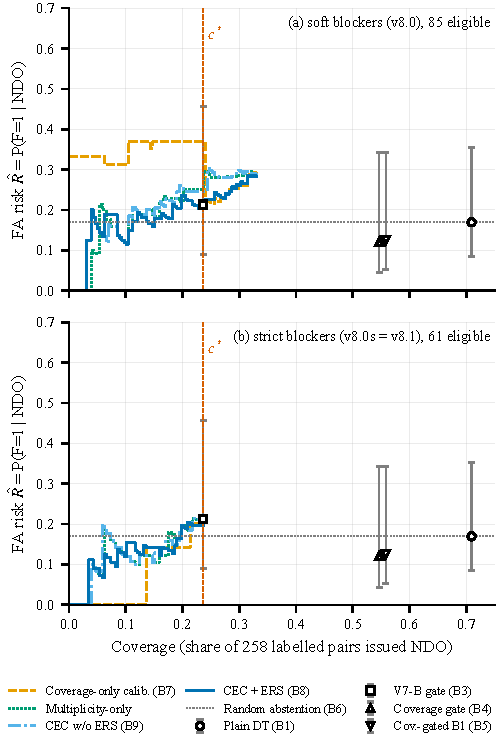
\includegraphics[width=\columnwidth]{figures/fig_risk_coverage.pdf}
\caption{Risk--coverage curves for the calibrated models (out-of-fold, seed 0) under soft and strict blocker policies, with rule baselines as points (95\% project-cluster bootstrap intervals). The vertical line marks $c^\ast=61/258$.}
\label{fig:riskcov}
\end{figure}

\begin{figure}[!t]
\centering
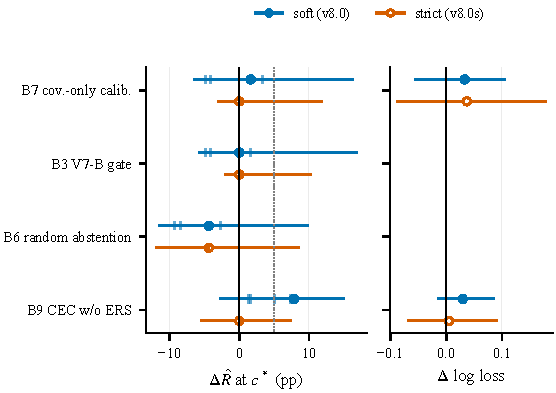
\includegraphics[width=\columnwidth]{figures/fig_ablation_forest.pdf}
\caption{Paired contrasts with full \cec{} (B8) at matched coverage (left, pp) and in out-of-fold log loss (right). Positive values favor B8. Dots: seed 0 with 95\% intervals; ticks: seeds 1--4. The dotted line marks the 5-pp margin of H2.}
\label{fig:forest}
\end{figure}

\paragraph*{RQ5: scope of the evaluation evidence}\label{sec:res-rq5} Five evaluation settings were executed in one language; apart from the single-run test split below, all are development data. The BugsInPy units are the only real-project changes. They have no labels, so they enter RQ2 and descriptive analyses but not the risk estimates. Under the predecessor's gate they received 6 \DIV{}, 8 \NDO{} and 32 \INS{} verdicts, an abstention rate of 70\%, against 48\% (127 of 266) in the synthetic and QuixBugs arms. The five-dataset artifact has 250 records from 12 hand-written templates, with commit identifiers that are SHA-1 digests of literal strings, 180 Java records that were not compiled or run, outcomes set from labels, and a stub predictor. It has no human verdicts (0 of 250), so it is invalid as external-validation evidence and is excluded. Cross-platform evidence shows that the analysis is reproducible. It does not show reproducible evidence collection on two platforms: the development records do not record the collection platform, and the Linux isolation results lack host metadata.

\paragraph*{Single-run test-split evaluation} The repository records one run of the frozen evaluation script on a separate v8 test split: 956 scored pairs from 22 programs (547 changed, 409 equivalent), after a pre-scoring exclusion of four programs. The split is not independent of the development data, since it shares its generator design with the development corpus, and the run was not replicated. The composite score \texttt{sbg\_v5} reached AUROC 0.694 (95\% cluster-bootstrap interval 0.659--0.727). Reversed edit size reached 0.876 (0.859--0.892), and two learned predictors reached 0.751 and 0.771. The paired difference between the composite score and reversed edit size was $-0.182$ ($-0.220$ to $-0.144$; Holm-adjusted $p=0.006$). Within exact edit-size strata the composite score reached AUROC 0.776 (0.722--0.825), above a label-shuffle noise floor with 95th percentile 0.528. The declared verdict is \emph{not demonstrated}: the stratified criterion was met, but the composite score did not beat the best baseline with an interval above zero. A post hoc component comparison, observed after this result, is exploratory and is not reported as a finding.

\section{Discussion and Threats to Validity}\label{sec:discussion}
About one in six plain no-difference outcomes concealed a labeled change, and about one in five of the predecessor gate's reassuring verdicts did. The magnitude depends on construction labels and small generated programs, so it does not transfer. What transfers is that abstention is not reliability: the gate issued a third as many verdicts as plain differential testing without lowering the rate of false assurance among them. Its apparent reduction from 31 to 13 false assurances follows almost entirely from issuing fewer verdicts (Proposition~\ref{prop:random}). Any proposal that withholds verdicts should report risk at matched coverage against random abstention. The ERS is useful as a conformance test. It found a profile defect that no aggregate metric revealed, distinguished stored from recomputed verdicts, and made the fitted model's dependence on one feature visible. These checks need no labels.

The data give no evidence of improvement, since no primary interval excludes zero. They give no evidence of no improvement, because the intervals admit advantages of up to 16 pp. They give no evidence of equivalence, which would require a pre-specified margin and an interval inside it; no such margin was declared. Three design facts further limit the predictive comparison: the fitted model keeps essentially one feature (multiplicity); provenance, integrity and environment were constant in training; and the influence feature is a reachability proxy, much weaker than checked coverage.

The corpus was not held out. The integrity-first ordering and the profile fix were both responses to ERS results on the same records, which favors \sbg{}; its predictive comparison remained negative. The corpus was examined repeatedly during design, and the labels are not adjudicated. In the QuixBugs arm the same declared inputs produce both label and evidence, so behavior-changing pairs almost always yield a witness, which understates risk there. The single-run test split is not an independent replication. Values were read from machine-readable outputs or from the source tables cited in the text; the cross-platform agreement figure is reported by the project and was not re-run. Threats are summarized in the supplementary material.

\section{Reproducibility and Data Availability}\label{sec:repro}
The project repository is public at \url{https://github.com/ManasSakthivel/Software-Behavior-Genome-SBG-Execution-Grounded-Behavioral-Representation}. The development records (\code{datasets/v8/dev\_records.jsonl}), the held-out test pairs (\code{artifacts/final/pairs\_v8test\_output\_free\_v8.jsonl}), the frozen threshold files (\code{artifacts/final/THRESHOLD\_FROZEN.json} and \code{artifacts/final/THRESHOLD\_V8\_FROZEN.json}), and the real-execution matrix with its manifests (\code{results/v8\_mac\_perturb/realexec\_matrix.json} and \code{results/v8\_mac\_perturb/realexec\_20261118/}) are on branch \code{research/v8-linux-validation}, which also contains the frozen implementation at commit \code{2edfe568}. Branch \code{research/v8-mac-hardening} (commits \code{8e28f601} and \code{b9b8a86c}) contains the macOS placebo, frozen-threshold and profile-fix results. The per-run execution directories behind the real-execution matrix are not in the repository. The security re-run output and its script are at \url{external_pilot/phase3_to_phase6/closeout/manuscript_final/audit/security_rerun_darwin.json} and \url{external_pilot/phase3_to_phase6/closeout/manuscript_final/scripts/audit_security_rerun.py} (commit \code{df612db0}). The statistics summary and recomputation script are at \url{external_pilot/phase3_to_phase6/closeout/manuscript_final/audit/stats_summary.json} and \url{paper/IEEE_ACCESS_V8_FINAL/scripts/stats_recompute.py}. The frozen snapshot and its SHA-256 checksums are in \url{external_pilot/phase3_to_phase6/phase3/}. The supplementary tables are at \url{external_pilot/phase3_to_phase6/closeout/manuscript_10page/supplement/tables.tex}.

Two frozen decision thresholds differ and the discrepancy is unresolved. The freeze manifest declares $\tau^\ast=0.072905$, and the held-out test record uses $\tau=0.040511$, derived on development data. Both values are preserved, and neither is claimed as the validated operating point. The frozen V8 test-suite run is incomplete: of 806 collected tests, 372 passed and none failed among those run; one test stalled and the run was stopped, and the remaining 433 were not run. This paper does not rely on that run.

\label{sec:conclusion}
An empty difference set is evidence that no divergence was observed on the inputs that were run, within the channels that were watched. We treated the corresponding verdict as a selective prediction, defined its false-assurance risk relative to a declared boundary and budget, separated it from equivalence, and showed that risk under a narrower boundary lower-bounds risk under a wider one. On 312 development pairs, plain differential testing gave false assurance in about one in six no-difference verdicts, and a gate that abstained heavily did not lower that rate. The ERS found a real profile defect that aggregate metrics missed. Whether richer evidence improves risk estimates remains open, and answering it requires an independently adjudicated external corpus of several hundred to over a thousand issued verdicts. No such evaluation has been carried out, and the single-run test-split result was not demonstrated.

\bibliographystyle{IEEEtran}
\bibliography{references}


\EOD
\end{document}
